\chapter{Quem cai primeiro}\label{cap:primeiro}

O capítulo anterior mediu a direção do tempo dentro de uma série. Falta a mesma pergunta no par:
quando as coisas ruins vêm juntas, alguém cai primeiro, e essa ordem se repete?

\section{A ordem que a proteção supõe}

O índice americano e o Ibovespa caem juntos muito mais do que a independência prevê ---
\numConjuntaExcesso{} vezes, medidos nos \numConjuntaDias{} dias em que as duas séries existem, com
\numConjuntaRompeA{} rompimentos de um lado, \numConjuntaRompeB{} do outro e \numConjuntaJuntos{} dias
em que os dois rompem ---, e \numConjuntaAcompanhados{} dos rompimentos de uma perna vêm com a outra
no mesmo dia. A leitura
natural de um número desses é que a queda conjunta é um acontecimento só, sem ordem interna: o dia
de uma perna encontra o dia da outra e pronto.

Se for assim, proteger uma perna não ajuda a outra nem atrapalha, porque não há intervalo entre as
duas quedas para fazer nada. A pergunta é se esse intervalo existe.

\section{A contagem}

O instrumento é uma contagem de episódios, e a regra precisa ser dita antes de ser usada.

\begin{definicao}[episódio dirigido]\label{def:episodio}
Um \emph{episódio} começa no dia em que uma das pernas rompe o próprio corte e nenhuma das duas
rompeu nos \numConjuntaJanelaEpisodio{} dias anteriores. O episódio é \emph{dirigido} quando a
outra perna rompe dentro dos dias seguintes à janela declarada, e a perna que rompeu primeiro é a
\emph{líder}. A \emph{assimetria} é a diferença entre os episódios liderados por uma perna e os
liderados pela outra, dividida pelo total de episódios dirigidos.
\end{definicao}

A regra tem um viés próprio, e escondê-lo seria medir a regra em vez do mundo: a espera olha para
trás e a detecção olha para a frente, de modo que num par sem adiantamento nenhum os dois lados não
saem iguais. Por isso o número do par real só vale contra o número dos pares sorteados, e nunca
contra zero --- é a mesma disciplina dos capítulos do orçamento e da direção.

Pelo mesmo motivo a inversão do relógio não serve de conferência aqui. No capítulo da direção ela
funcionou, porque a estatística de lá não tinha regra nenhuma dentro; aqui a regra é assimétrica, e
virar o mundo ao contrário não a vira junto. Quem confere este instrumento é o nulo, que carrega a
mesma regra.

\section{O nulo, e o par}

Medindo \numConjuntaNulos{} pares sorteados e contemporâneos com a mesma regra, a assimetria tem
média \numConjuntaNuloMedia{} e dispersão \numConjuntaNuloDispersao{}. A média é praticamente zero,
e o motivo dela tem história: a primeira versão desta contagem tratava o rompimento simultâneo como
episódio de uma das pernas, e isso inventava direção onde não havia nenhuma. Um dia em que as duas
caem juntas não tem primeiro.

Contra esse nulo, o par como veio faz o seguinte.

\begin{table}[htbp]
  \centering
  \small
  \begin{tabular}{rrrr}
    \hline
    janela do & episódios & episódios & assimetria \\
    episódio & liderados pelo índice & liderados pelo Ibovespa & medida \\
    \hline
    um & \numConjuntaLiderAUm & \numConjuntaLiderBUm & \numConjuntaAssimetriaUm \\
    cinco & \numConjuntaLiderACinco & \numConjuntaLiderBCinco & \numConjuntaAssimetriaCinco \\
    dez & \numConjuntaLiderADez & \numConjuntaLiderBDez & \numConjuntaAssimetriaDez \\
    vinte e um & \numConjuntaLiderAVinteEUm & \numConjuntaLiderBVinteEUm & \numConjuntaAssimetriaVinteEUm \\
    \hline
  \end{tabular}
  \caption{Os episódios dirigidos no par, por janela. A janela é quanto tempo se espera pela
    segunda perna depois de a primeira ter rompido.}
  \label{tab:episodios}
\end{table}

Na janela de \numConjuntaJanelaEpisodio{} dias o índice lidera \numConjuntaLiderA{} episódios e o
Ibovespa lidera \numConjuntaLiderB{}, o que dá uma assimetria de \numConjuntaAssimetria{} ---
\numConjuntaDesvios{} desvios acima do nulo. O número é positivo em todas as janelas testadas, e
não é pequeno.

\section{Quanto dura o adiantamento}

A assimetria diz que existe uma ordem; ela não diz de quanto tempo é o intervalo. Para medir isso, o
instrumento é posto à prova contra um adiantamento declarado: a segunda perna é deslocada dia a dia
e a assimetria é remedida.

\begin{figure}[htbp]
  \centering
  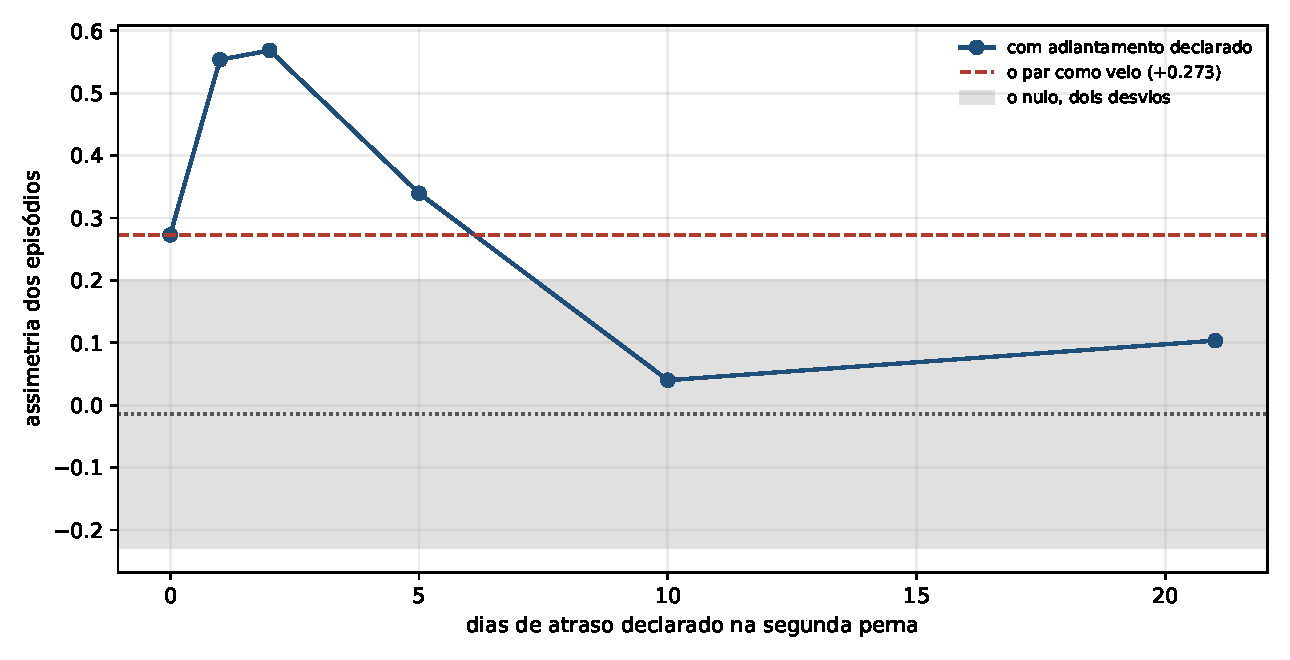
\includegraphics[width=\linewidth]{figuras/E14_direcao_conjunta_1.pdf}
  \caption{A assimetria contra o atraso declarado na segunda perna. A faixa cinza é o nulo a dois
    desvios, a linha tracejada é o par como veio, e a curva mostra onde o par se alinha melhor.}
  \label{fig:adiantamento}
\end{figure}

A curva sobe antes de descer. Sem deslocamento nenhum a assimetria é \numConjuntaControleZero{}.
Com a segunda perna deslocada em um ou dois dias, ela chega ao seu máximo ---
\numConjuntaControleUm{} e \numConjuntaControleDois{} ---, acima do valor do par como veio. Com
cinco dias cai para \numConjuntaControleCinco{}, com dez dias para \numConjuntaControleDez{}, e com
\numConjuntaAtrasoMaior{} dias para \numConjuntaControleVinteEUm{}, dentro da faixa do nulo.

Vale dizer o que o eixo faz. Os seis pontos medidos --- zero, um, dois, cinco, dez e vinte e um dias
--- estão igualmente espaçados no desenho: o passo do primeiro para o segundo vale um dia, e o dos
dois últimos vale onze, com a mesma largura. Quem lê a inclinação entre os dois pontos da direita lê
onze dias como se fossem um.

Isso localiza o adiantamento: o par se alinha melhor quando o índice lidera por um ou dois dias. É
esse o intervalo de que uma proteção dispõe entre o rompimento de uma perna e o da outra, e é ele
que decide se há alguma coisa a fazer no meio.

\section{Se repete}

Uma direção medida uma vez é um episódio do dado, e não uma propriedade dele. A conferência é
partir o par em pedaços e medir cada um.

\begin{figure}[htbp]
  \centering
  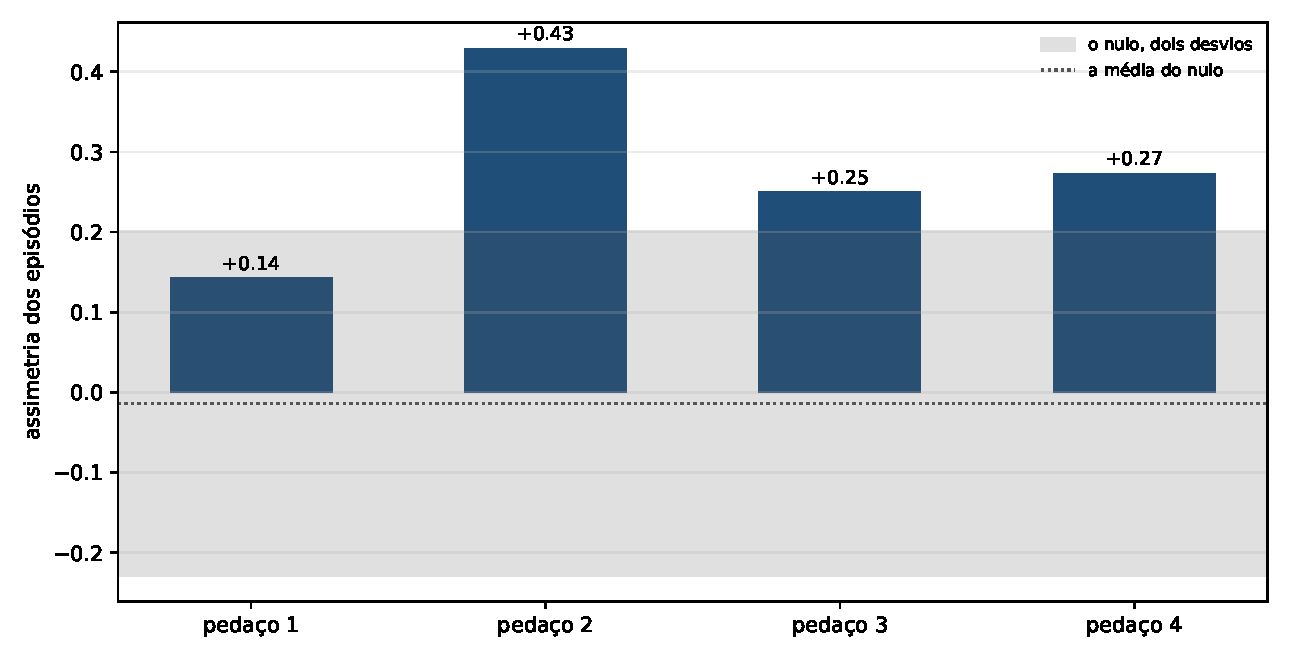
\includegraphics[width=\linewidth]{figuras/E14_direcao_conjunta_2.pdf}
  \caption{A assimetria em cada pedaço do par, contra a faixa do nulo. Os quatro pedaços têm
    \numConjuntaPrimeiroDias{}, \numConjuntaSegundoDias{}, \numConjuntaTerceiroDias{} e
    \numConjuntaQuartoDias{} dias.}
  \label{fig:pedacos}
\end{figure}

Os quatro pedaços dão \numConjuntaPrimeiroAssimetria{}, \numConjuntaSegundoAssimetria{},
\numConjuntaTerceiroAssimetria{} e \numConjuntaQuartoAssimetria{}: todos positivos, e
\numConjuntaPedacosAcima{} de \numConjuntaPedacos{} acima da média do nulo. O sinal se repete. O
tamanho varia bastante de pedaço para pedaço, e o motivo está na contagem: os quatro pedaços têm
\numConjuntaPrimeiroLiderA{}, \numConjuntaSegundoLiderA{}, \numConjuntaTerceiroLiderA{} e
\numConjuntaQuartoLiderA{} episódios dirigidos liderados pelo índice, e com tão poucos episódios cada
pedaço, sozinho, não distingue nada.

\section{O que fica}

Fica a resposta da travessia, e ela é um sim com medida. A perda conjunta tem direção: o índice cai
primeiro, o Ibovespa vem atrás num ou dois dias, e a ordem se repete nos quatro pedaços do dado. O
A precisão fica de fora. O efeito é de \numConjuntaDesvios{} desvios sobre o total do
par, cada pedaço isolado é fraco, e a regra de contagem não pode ser conferida pelo relógio
invertido, porque a regra ela mesma tem lado.

Fica também o que a travessia inteira mostrou, olhando para trás. Cinco perguntas medidas com o
instrumento de outra família, e as cinco deram o mesmo tipo de resposta: existe sinal, e o sinal
custa --- em dias de experimento, em trabalho de atualização, em passado apagado, em anos de espera.
Cada capítulo desta travessia terminou com um preço medido, e nenhum deles terminou com uma
promessa que a conta prometia e o mundo não pagava.

O que sobra é a pergunta que a travessia deixa de pé ao terminar. Quase tudo o que a espiral mediu
até aqui se compra: memória se compra com dias, atualização se compra com trabalho, um experimento
se compra com replicatas. A espiral vira agora para o outro lado da mesma conta, e a pergunta do
movimento seguinte é o que \textbf{não} se compra de jeito nenhum --- começando pela mais dura de todas,
que é o mundo que não foi observado.
